\documentclass[12pt]{article}
\usepackage{amsmath, amssymb, graphicx, tikz, geometry}
\geometry{margin=1in}
\usepackage{newunicodechar}
\newunicodechar{ℵ}{\ensuremath{\aleph}}

\title{Discrete Mathematics for Young Puzzle Masters}
\author{Compiled Stories of Great Mathematicians}
\date{}

\begin{document}

\newpage

\section*{Chapter 1: The Story of Discrete Mathematics}

\subsection*{Introduction: From Ancient Puzzles to Modern Cubes}

Mathematics is like a grand story, where each chapter introduces new characters (the mathematicians) and exciting ideas. \textbf{Discrete mathematics} is the branch of math that deals with things we can count or list step by step, as opposed to smooth continuous things like curves in calculus. In discrete math, we study objects like whole numbers, puzzles, or logical statements that are \emph{separate and distinct}. This story of discrete math spans \textbf{thousands of years}, beginning with ancient thinkers and leading all the way to modern puzzles like the \textbf{Rubik’s Cube}.

Imagine \emph{counting} rocks or solving a puzzle one move at a time – that’s discrete math! It includes \emph{set theory} (the study of collections of things), \emph{logic} (the rules of true and false), \emph{algebra} (using symbols to stand for numbers), and \emph{group theory} (the mathematics of symmetry and moves, like twisting a Rubik’s Cube). Discrete math might sound complex, but it’s something even young mathematicians can explore step by step.

Before we dive into history, let’s meet some special characters that mathematicians use: \textbf{Greek letters}! Mathematicians often use the Greek alphabet (\(\alpha, \beta, \gamma, \dots, \pi, \Sigma, \Omega\)) to represent numbers or concepts. For example, the letter \(\pi\) (“pi”) is about \(3.14159\ldots\) and represents the ratio of a circle’s circumference to its diameter. We will explain each Greek letter when it appears.

\subsection*{Euclid and the Birth of Reasoning (300\,BC)}

Euclid lived in Alexandria, Egypt, around 300\,BC. He wrote \emph{Elements}, collected existing geometry, and presented the first recorded \emph{algorithm}—the Euclidean algorithm for finding the greatest common divisor (GCD) of two integers.

Find the GCD of \(a=28\) and \(b=21\):
\[
\gcd(28,21)=\gcd(21,28-21)=\gcd(21,7)=7.
\]

Euclid pioneered rigorous \emph{proof} and logical deduction, the backbone of mathematics.

\subsection*{Euler and the Seven Bridges Puzzle (1736)}

Leonhard Euler (1707–1783) solved the Seven Bridges of Königsberg puzzle by abstracting the map into a \emph{graph} with vertices and edges. He proved no walk crosses each bridge exactly once and thereby founded \emph{graph theory}. Graphs now help route internet traffic, plan trips, and analyze puzzles.

\subsection*{Gauss and Clever Summations (1790s)}

Young Carl Friedrich Gauss (1777–1855) amazed his teacher by summing integers \(1\) to \(100\) instantly:
\[
\sum_{i=1}^{100} i = 50 \times 101 = 5050.
\]

Gauss later developed \emph{modular arithmetic}. We write \(13 \equiv 1 \pmod{12}\) to show 13 leaves remainder 1 when divided by 12.

\subsection*{Galois and the Invention of Group Theory (1830)}

Évariste Galois (1811–1832) explored why general quintic equations have no simple formula. He associated to each polynomial a \emph{group} of permutations of its roots. His overnight letters created modern \emph{group theory}. The Rubik’s Cube group, a non‑abelian group of face twists, is a direct descendant of Galois’s ideas.

\subsection*{Boole and Algebra of Logic (1854)}

George Boole (1815–1864) published \emph{The Laws of Thought}, introducing Boolean algebra with values \(0\) (false) and \(1\) (true). Boolean operations (\(\land\), \(\lor\), \(\lnot\)) underpin digital circuits and programming.

\subsection*{Cantor and the Infinite Universe of Sets (1874)}

Georg Cantor (1845–1918) founded set theory and showed infinities come in different sizes. He proved the set of real numbers is \emph{uncountable}. Cantor introduced symbols like \(\aleph_0\) for the cardinality of natural numbers and \(\omega\) for the first infinite ordinal.

\subsection*{Why These Stories Matter for Puzzles}

The Rubik’s Cube has \(43\,252\,003\,274\,489\,856\,000\) configurations. Understanding sets, permutations, logic, and group structure lets us design algorithms that solve any scramble in at most 20 moves (“God’s Number”).

\newpage
\section*{Chapter 2: Group Theory and the Rubik's Cube}

\subsection*{Introduction}

In Chapter 1 we met the Rubik’s Cube and the great minds of history. Now we dive into the secret language that describes every twist and turn: \textbf{group theory}. Imagine a secret code that tells you exactly how each move reshuffles the cube’s colored stickers.

\subsection*{What Is a Group?}

A \emph{group} is a set \(G\) with an operation \(\ast\) satisfying:
\begin{enumerate}
  \item \textbf{Closure}: \(a,b\in G \Rightarrow a\ast b\in G\).
  \item \textbf{Associativity}: \((a\ast b)\ast c = a\ast(b\ast c)\).
  \item \textbf{Identity}: \(\exists e\in G\) s.t. \(e\ast a=a\ast e=a\).
  \item \textbf{Inverse}: \(\forall a\in G, \exists a^{-1}\in G\) with \(a\ast a^{-1}=e\).
\end{enumerate}

\subsection*{The Rubik’s Cube as a Group}

Let \(M\) be the set of all face twists. Composition \(\,\circ\,\) of moves makes \((M,\circ)\) a group. The solved cube is the identity element; each twist has an inverse.

\subsection*{Permutations and Cycle Notation}

Sticker positions form a set \(S\). A move is a permutation \(\sigma:S\to S\). Example:
\[
(1\;3\;9\;7)(2\;6\;8\;4)
\]
means \(1\to3\to9\to7\to1\) and \(2\to6\to8\to4\to2\).

\subsection*{Worked Example: A Face Turn}

Label front stickers \(1\)–\(9\). A \(90^\circ\) clockwise turn is
\[
(1\;3\;9\;7)(2\;6\;8\;4).
\]
Its inverse (counter‑clockwise) reverses each cycle.

\subsection*{Why This Matters}

Group theory lets us craft algorithms that move certain cubies while leaving others fixed, leading to efficient solutions.

\section*{Chapter 3: The Tesseract—Exploring Four Dimensions}

\subsection*{Introduction: Why Go Beyond 3D?}
We live in a three–dimensional (3D) world: every object has \emph{length}, \emph{width}, and \emph{height}. Mathematics lets us imagine spaces with more dimensions. The simplest 4–dimensional (4D) shape analogous to a cube is called a \textbf{tesseract}. Understanding it sharpens mental geometry skills that help with higher–order puzzles like the 4D Rubik’s Cube simulator \emph{MagicCube4D}.

Before we begin, we introduce two more Greek letters. The letter $\theta$ (theta) will denote a rotation \emph{angle}, and $\xi$ (xi) will represent a fourth coordinate. Every symbol will be defined on first use.

\subsection*{Counting Dimensions With Powers of Two}
For an $n$–dimensional cube (also called an \emph{$n$–hypercube}), the number of vertices is $2^{n}$.  For example:
\begin{itemize}
  \item 0D (a point): $2^0 = 1$ vertex.
  \item 1D (a line segment): $2^1 = 2$ vertices.
  \item 2D (a square): $2^2 = 4$ vertices.
  \item 3D (a cube): $2^3 = 8$ vertices.
  \item \textbf{4D (a tesseract):} $2^4 = 16$ vertices.
\end{itemize}

\paragraph{Example.}  Label the 4D coordinates of a tesseract’s vertices using $(x, y, z, \xi)$ where each coordinate is either $0$ or $1$.  The vertex $(0,0,0,0)$ is one “corner,” and $(1,1,1,1)$ is the opposite “corner” four units away through 4D space.

\subsection*{Projecting 4D Into 3D and 2D}
Since humans cannot see 4D directly, we \emph{project} it into 3D (and then onto 2D paper or screens).  A common method is the \emph{Schlegel diagram}.  Imagine shining a light through the tesseract so its “shadow” lands inside a 3D cube.  The result looks like a small cube nested inside a larger cube, with edges connecting matching vertices.

\begin{center}
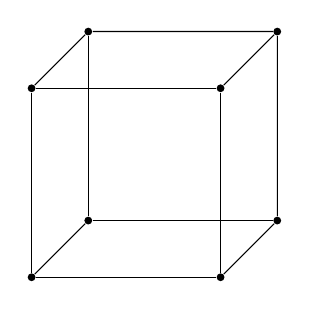
\begin{tikzpicture}[scale=1.2, every node/.style={circle, fill=black, inner sep=1pt}]
  % outer cube vertices
  \foreach \x/\y in {0/0, 2/0, 2/2, 0/2} \node (o\x\y) at (\x,\y) {};
  % inner cube vertices (shifted)
  \foreach \x/\y in {0/0, 2/0, 2/2, 0/2} \node (i\x\y) at (\x+0.6,\y+0.6) {};
  % outer cube edges
  \foreach \a/\b in {o00/o20,o20/o22,o22/o02,o02/o00} \draw (\a) -- (\b);
  % inner cube edges
  \foreach \a/\b in {i00/i20,i20/i22,i22/i02,i02/i00} \draw (\a) -- (\b);
  % connecting edges
  \foreach \a/\b in {o00/i00,o20/i20,o22/i22,o02/i02} \draw (\a) -- (\b);
\end{tikzpicture}
\end{center}
\vspace{-0.5em}
\emph{Figure:} A Schlegel projection of a tesseract (outer cube linked to inner cube).

\subsection*{Rotation Matrices in Four Dimensions}
In 3D we rotate around an \emph{axis}. In 4D we rotate within a \emph{plane}. There are six coordinate planes: $xy$, $xz$, $yz$, $x\xi$, $y\xi$, and $z\xi$.  A rotation by an angle $\theta$ in the $x\xi$–plane is represented by the matrix
\[
R_{x\xi}(\theta)=
\begin{bmatrix}
\cos \theta & 0 & 0 & -\sin \theta\\
0 & 1 & 0 & 0\\
0 & 0 & 1 & 0\\
\sin \theta & 0 & 0 & \cos \theta
\end{bmatrix}.
\]
Here $\theta$ (Greek letter theta) is measured in radians.  Multiplying this matrix by the coordinate column vector $(x, y, z, \xi)^{T}$ produces the rotated point.

\paragraph{Worked Example.} Rotate the point $(1,0,0,0)$ by $\theta=\frac{\pi}{2}$ (\(90^{\circ}\)) in the $x\xi$–plane:
\[
R_{x\xi}\!\bigl(\tfrac{\pi}{2}\bigr)\!
\begin{bmatrix}1\\0\\0\\0\end{bmatrix}
=
\begin{bmatrix}0\\0\\0\\1\end{bmatrix}.
\]
The $x$–coordinate becomes $0$, and the hidden $\xi$–coordinate becomes $1$ after rotation.

\subsection*{From Tesseract to a 4D Rubik’s Cube}
Software such as \emph{MagicCube4D} implements a $3\times3\times3\times3$ hypercube puzzle. Each “face turn” in 4D is a 3D slice rotation.  The total number of configurations is gigantic—on the order of $10^{120}$.  Solving such a puzzle requires understanding \emph{commutators} and \emph{conjugates}—two group–theoretic tools we will meet in Chapter 4.

\subsection*{Key Takeaways}
\begin{itemize}
  \item Vertex counts of hypercubes follow $2^{n}$.
  \item 4D rotations occur in planes and are described by $4\times4$ matrices.
  \item Projections like the Schlegel diagram help us visualise 4D objects.
  \item The 4D Rubik–style puzzle generalises cube–solving strategies to higher dimensions.
\end{itemize}

In the next chapter we will design \textbf{algorithms} that manipulate a tesseract puzzle—moving pieces precisely while keeping most of the structure fixed, just like on the classic 3D cube.

\end{document}
